\documentclass[a4,paper,fleqn]{article}

\usepackage{layout}

\DeclareSIUnit\year{Jahr}

\title{Notizen EEV -- SW06}
\date{\today}
\author{Daniel Winz}

\begin{document}
\maketitle
\clearpage

\section{Impulssatz eulersche Hauptgleichung}
Impuls: 
\[ F \cdot dt = m \cdot dv \]
Annahme: 
\[ dt = 1 \si{\second} \]
\[ F = Q \cdot \varrho \cdot \Delta v \]
\[ F_{Turb} = Q \cdot \varrho (v_{Eintritt} - v_{Austritt}) \]
Merke! Abgegebene Kraft an der Turbinenschaufel resp. Pumpenschaufel gleich 
der Impulsdifferenz zwischen Druck- und Saugkante! 

\subsection{Hydraulisches Moment}
\[ \text{Leistung} = \text{Moment} \cdot \text{Winkelgeschwindigkeit} \]
\[ M_{Hyd} = Q \cdot \varrho \cdot (R_1 \cdot v_1 - R_2 \cdot v_2) \]
\[ P_{Hyd} = M_{Hyd} \cdot \omega \]
\[ P_{Hyd} = Q \cdot \varrho \cdot \omega \cdot (R_1 \cdot v_1 - R_2 \cdot v_2) \]

\section{Diffusor}
$\Rightarrow$ Energiewandler \\
Umwandlung von kinetischer Energie in statische Druckenergie
\\
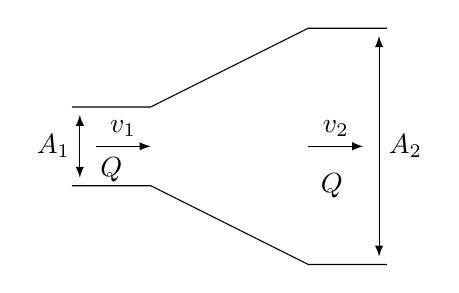
\begin{tikzpicture}
    \draw (0,3) -- (1,3) -- (3,4) -- (4,4);
    \draw (0,2) -- (1,2) -- (3,1) -- (4,1);
    \draw[latex-latex] (0.1,2.1) -- node[left]  {$A_1$} (0.1,2.9);
    \draw[latex-latex] (3.9,1.1) -- node[right] {$A_2$} (3.9,3.9);
    \draw[-latex] (0.3,2.5) -- node[above] {$v_1$} (1.0,2.5);
    \draw[-latex] (3.0,2.5) -- node[above] {$v_2$} (3.7,2.5);
    \node at (0.5,2.2) {$Q$};
    \node at (3.3,2.0) {$Q$};
\end{tikzpicture}
\\
\[ g \cdot h + \frac{p}{\varrho} + \frac{v^2}{2} = \text{const} \]
(Ohne Reibungsverluste)
\[ p_1 + \frac{\varrho \cdot {v_1}^2}{2} + \varrho \cdot g \cdot h_1 
= p_2 + \frac{\varrho \cdot {v_2}^2}{2} + \varrho \cdot g \cdot h_2  \]
\[ Q = A_1 \cdot v_1 = A_2 \cdot v_2 \]
\[ p_2 = p_1 + \frac{\varrho \cdot {v_1}^2}{2} \cdot \left( 1 - \frac{{A_1}^2}{{A_2}^2} \right) \]

\section{Verluste und Begriffe}
\begin{itemize}
    \item Natürliche hydraulische Leistung
        \[ P_{nat} = Q \cdot \varrho \cdot g \cdot H_{br} \]
    \item Verfügbare disponible Leistung
        \[ H_{net} = H_{br} - H_{v} \]
        $H_{v} \equiv$ Verluste im Triebwassersystem, z.B. Druckleitung, 
        Rechen usw. 
        \[ P_{disp} = Q \cdot \varrho \cdot g \cdot H_{net} \]
    \item Turbinenleistung (Wellenleistung)
        \[ P_{Turb} = Q \cdot \varrho \cdot g \cdot H_{net} \cdot \eta_{T} \]
    \item Generatorleistung (Leistungsabgabe ab Generator)
        \[ \boxed{P_{Abgabe} = Q \cdot \varrho \cdot g \cdot H_{net} \cdot \eta_{T} \cdot \eta_{G}} \]
\end{itemize}
\[ \Delta p_v = \lambda \cdot \frac{l}{d} \cdot \frac{\varrho}{2} \cdot v^2 \]

\end{document}
